\chapter{Estudio (preliminar) de las Incertezas Sistemáticas}\label{Syst}

La elección de algunos valores al momento de realizar selecciones de eventos es, de cierta manera, arbitraria. Si bien, por ejemplo, la decisión del umbral tanto para el criterio de aislación como para el matching está motivada por argumentos de geometría, no deja de ser una elección. Por lo tanto, se debe estudiar el impacto de realizar variaciones sobre estos parámetros en la calibración derivada, obteniéndose así las incertezas sistemáticas de este método. Un resumen de las incertezas sistemáticas estudiadas en esta tesis se presenta en la tabla \ref{tab:syst}


\begin{table}[ht]
    \centering
    \begin{tabular}{|l|l|l|} 
        \hline
        %\multicolumn{2}{|c|}{input} & \multicolumn{2}{c|}{output} & \\
        Sistemático & Descripción & Variación \\ \hline\hline
        \textbf{Muones} & &\\
        Escala & Incerteza en la escala de energía de los muones & $\pm 1\sigma$\\
        Resolución (ID) &  Incerteza en la resolución del momento de los & $\pm 1\sigma$\\
        & en el ID & \\ \hline
        \textbf{Método de} & &\\
        \textbf{Direct-Matching} &  &\\ 
        JES & Incerteza en la escala de energía de los Ref. Jets & $\pm 1\sigma$\\ 
        JVT & Incerteza en la discriminación de pile-up jets & 0.11 $(\downarrow)$ 0.91 $(\uparrow)$ \\
        Jets aislados ($f$) & $\Delta R> f*R$ & $f=$ 1.5$(\downarrow)$, 2.5$(\uparrow)$ \\
        $p_{t,\%}$ & relación de momento en aislación de jets & 5$\%(\downarrow)$ $20\%(\uparrow)$ \\
        Matching ($dR$) & $\Delta R(jet^{Rscan},jet^{Ref})<dR$ & $dR=$ 0.1$(\downarrow)$, 0.3$(\uparrow)$ \\ \hline 
        \textbf{Generador de MC}& Diferencia entre generadores de MC & Sherpa \\ \hline 
        \end{tabular}
    \caption{Resumen de incertezas sistemáticas estudiadas para las calibraciones R-scan en eventos de $Z+jets$.}
    \label{tab:syst}
\end{table}


En este trabajo, se estudiaron variaciones sistemáticas sobre los parámetros mencionados en la tabla \ref{tab:syst}, a valores por encima y por debajo del utilizado en la derivación de la calibración. Estos parámetros están directamente relacionados con el método utilizado, el método de direct-matching. Para el caso del parámetro JVT, las variaciones propuestas en la tabla \ref{tab:syst} corresponden a $\pm 1\sigma$ en la discriminación de pile-up jets y surgen de recomendaciones dadas en la ref. \cite{JVTtool}. 

Además de los sistemáticos asociados a cortes cinemáticos, se tienen que tener cuenta sistemáticos heredados de pasos anteriores a la aplicación del método de direct-matching, por ejemplo, incertezas asociadas a la identificación y corrección del momento de los muones. Estas variaciones también se corresponden a variaciones de $\pm 1\sigma$ según las recomendaciones dadas por el grupo CP de ATLAS en la ref. \cite{MCPGuidelines}. 

La elección del MC es otro factor que debe estudiarse. Como se mencionó en la sección \ref{predictions}, distintos generadores de MC (o combinaciones de ellos) simulan los eventos de maneras diferentes desde el elemento de matriz considerado, o el orden de la predicción, hasta el modelado del pile-up, el evento subyacente, las PDFs, la fragmentación y la hadronización. Entonces, con el fin de estudiar qué pasaría si se hubiera derivado la calibración con otra muestra de MC, en este trabajo se introduce una segunda muestra generada en Sherpa según se especifica en la sección \ref{Muestras}. 

Para todas las variaciones mencionadas arriba, el procedimiento utilizado para derivar las incertezas sistemáticas fue el mismo. Para cada parámetro se proponen dos variaciones, una por encima y una por debajo del valor utilizado; y para cada variación se vuelve a derivar una corrección tal y como se explica en la sección \ref{Derivandow}, manteniendo las otras fijas en el valor nominal.

En el caso de la elección de MC, se cuenta con una sola muestra extra a parte de la nominal. En particular, como ya se discutió en la sección \ref{Derivandow}, la muestra de Sherpa resultó tener poca estadística por lo que la corrección derivada con la misma presenta muchas fluctuaciones sustanciales.

Una vez obtenidas las correcciones a partir de estos parámetros variados, se las suaviza, y para cada bin de $p_t$ se calcula la diferencia relativa entre la corrección ``variada'' y la nominal. Una aclaración, quizás evidente, es que una variación de un parámetro  a un valor por encima del nominal no necesariamente se traduce en una variación de la corrección monótonamente hacia arriba, o hacia abajo, sino que la calibración correspondiente a la variación por encima de un dado parámetro puede encontrarse para algunos bines de momento por encima de la nominal y para otros por debajo. Por este motivo, y con el fin de simetrizar la incerteza a derivar, se guarda como contribución del parámetro, la diferencia relativa (al nominal) máxima, en valor absoluto, de las dos variaciones. 

En este punto se incorpora también una incerteza asociada a la calibración de los Ref Jets. Ésta es la incerteza de la JES estudiada en la referencia \cite{JESpaper}, que se corresponde con la incerteza total en la cadena completa de calibración para jets reconstruidos con el algoritmo anti-k$_t$ $R=$0.4 a partir de la escala EM. Esta incerteza fue proporcionada por el grupo de JetEtmiss de ATLAS.

La incerteza sistemática (relativa) total se obtiene de sumar las contribuciones de cada parámetro en cuadratura para cada bin de $\eta$ y $p_t$. 
En la figura \ref{fig:Un} se observa la incerteza sistemática (relativa) total (en negro), en función del momento transverso del jet, y las contribuciones de cada parámetro estudiado a la misma, para dos bines de $\eta$ y para ambas colecciones de Rscan Jets. De la misma se observa que la contribución más significativa es la incerteza de las JES en primera medida, y la asociada a la elección del MC. Las incertezas asociadas a la identificación y  corrección de momento de los muones, y la de JVT son insignificantes (menores al 0.4$\%$) frente a la contribución de la JES, la cual alcanza el 5$\%$ a bajo momento y decrece hasta el 2$\%$ hacia el extremo del rango de momento considerado. En las figuras \ref{fig:Un} (b) y (d) correspondientes al bin 2.4$<\eta^{Rscan}_{det}<$2.5 el hecho de que las curvas se vuelvan chatas en los últimos bines de momento no es representativo de la incerteza, sino de que en esos bines no se cuenta con calibración. 
La incerteza sistemática (relativa) total es del orden del 5$\%$ por debajo de los 30 GeV, y disminuye al 2$\%$ al llegar a los 200GeV.


\begin{figure}[ht]
    \centering
    \begin{subfigure}[b]{0.495\textwidth}
        \centering
        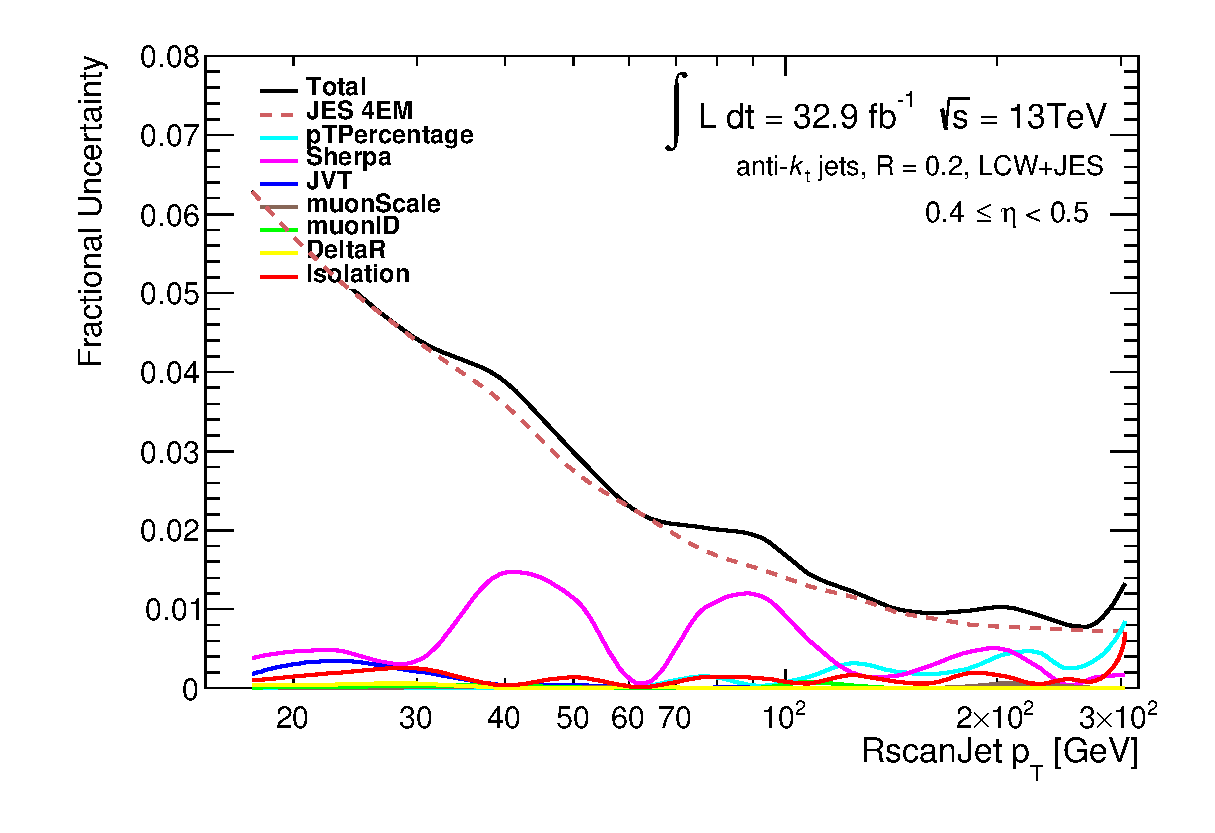
\includegraphics[width=\textwidth]{images/SumIn2_Eta_49_2LC_wContributions.eps}
        \caption{$R=$0.2 ; 0.4$<\eta^{Rscan}_{det}<$0.5}
        %\label{fig:data2lc49}
    \end{subfigure}
    \hfill
    \begin{subfigure}[b]{0.495\textwidth}
        \centering
        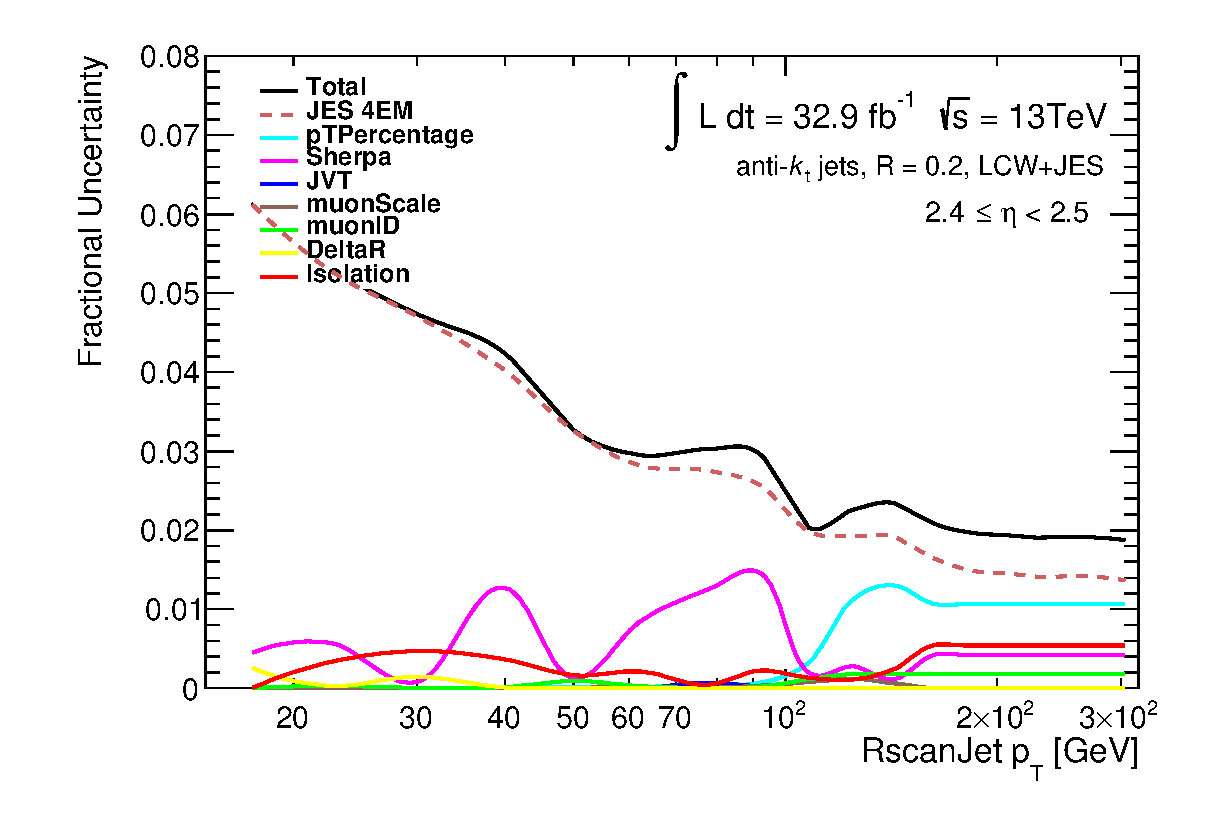
\includegraphics[width=\textwidth]{images/SumIn2_Eta_69_2LC_wContributions.eps}
        \caption{$R=$0.2 ; 2.4$<\eta^{Rscan}_{det}<$2.5}
        %\label{fig:Th26lc}
    \end{subfigure}
    \vfill
    \begin{subfigure}[b]{0.495\textwidth}
        \centering
        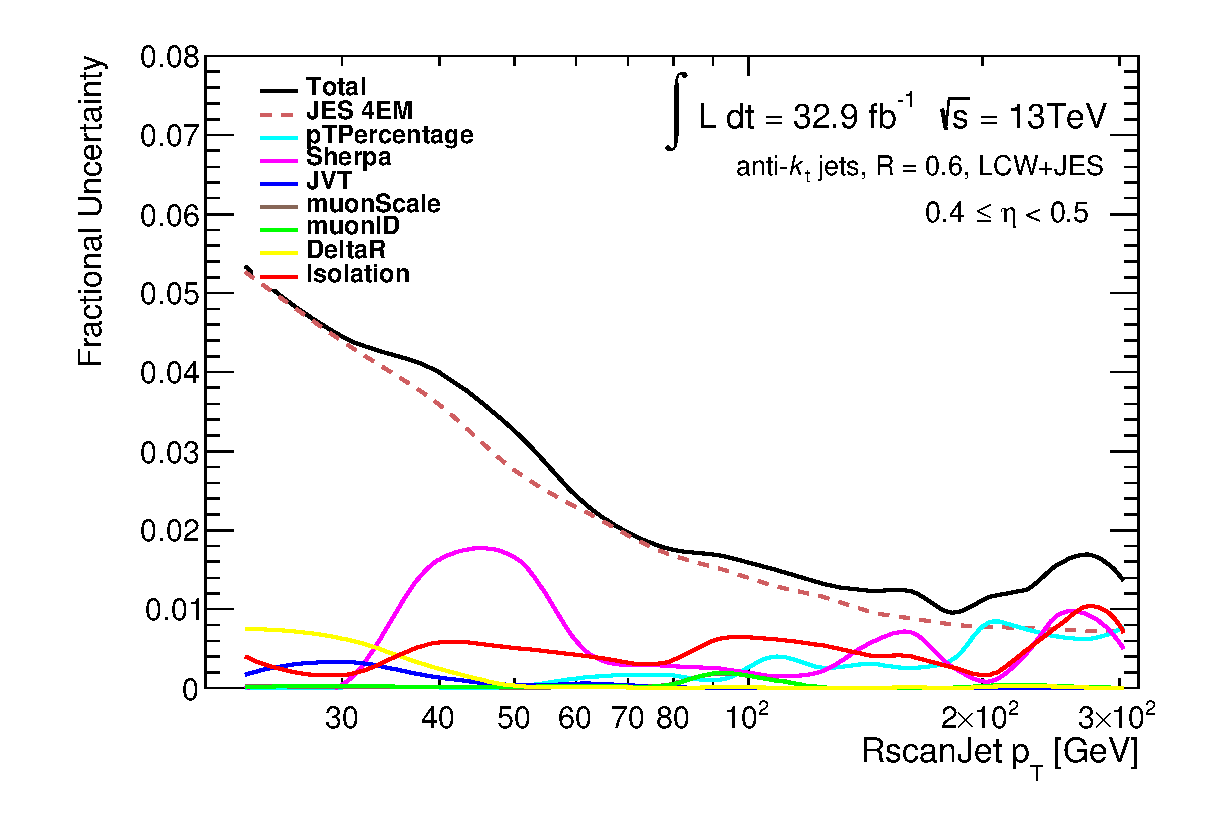
\includegraphics[width=\textwidth]{images/SumIn2_Eta_49_6LC_wContributions.eps}
        \caption{$R=$0.6 ; 0.4$<\eta^{Rscan}_{det}<$0.5}
        %\label{fig:fitFeo}
    \end{subfigure}
    \hfill
    \begin{subfigure}[b]{0.495\textwidth}
        \centering
        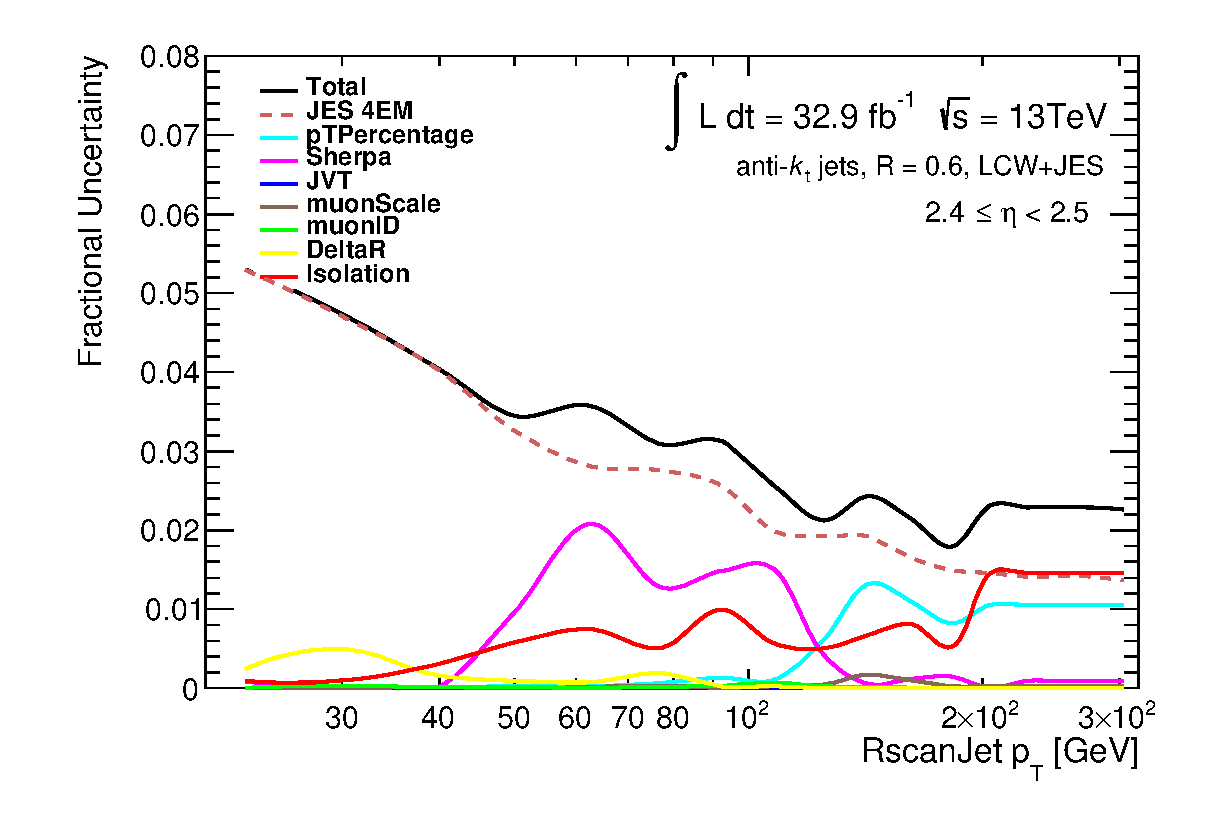
\includegraphics[width=\textwidth]{images/SumIn2_Eta_69_6LC_wContributions.eps}
        \caption{$R=$0.6 ; 2.4$<\eta^{Rscan}_{det}<$2.5}
        %\label{fig:Th26lc}
    \end{subfigure}
    \caption{ Incerteza Sistemática relativa total, en negro, y sus distintas contribuciones en función de $p_t^{Rscan}$, en bines de 0.4$<\eta^{Rscan}_{det}<$0.5 a la izquierda y de 2.4$<\eta^{Rscan}_{det}<$2.5 a la derecha. Las figuras de arriba corresponden a la colección de Rscan Jets con $R=$0.2 y las de abajo con 0.6. } 
    \label{fig:Un}
\end{figure}


\begin{figure}[ht]
    \centering
    \begin{subfigure}[b]{0.495\textwidth}
        \centering
        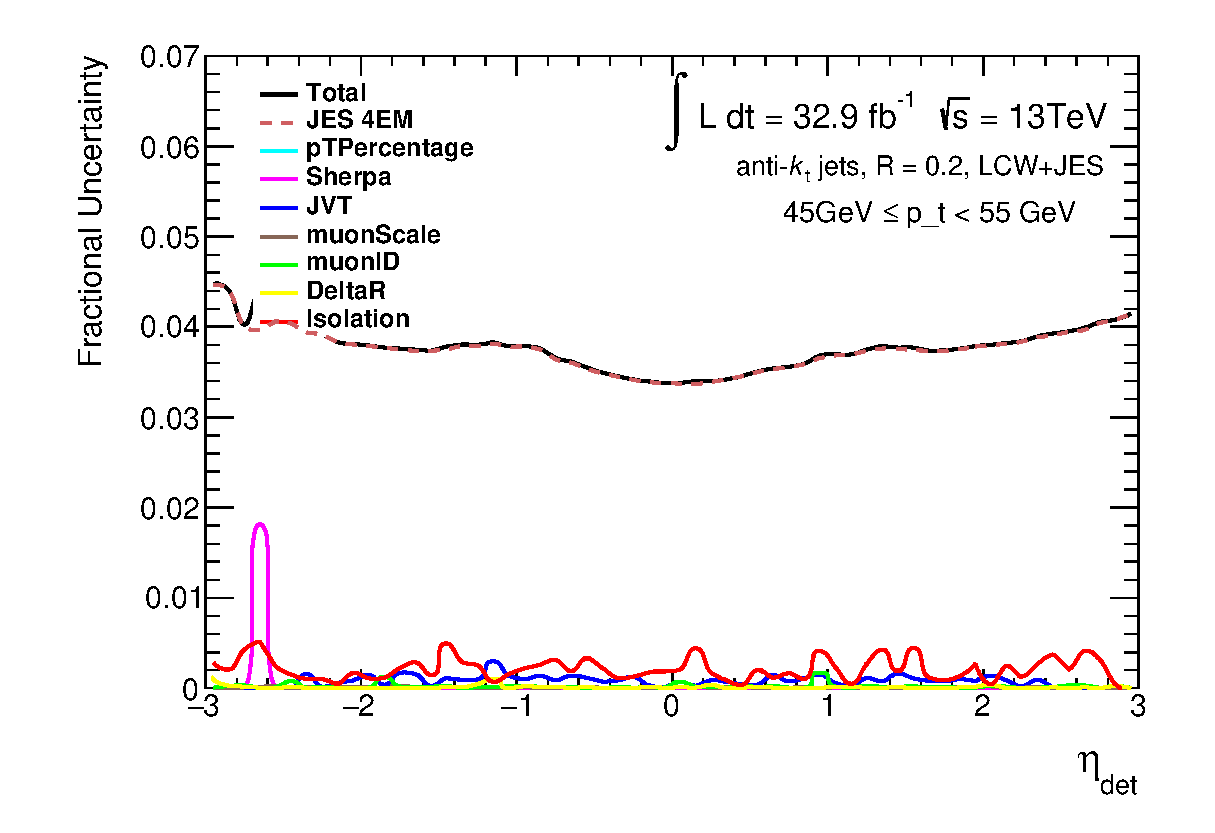
\includegraphics[width=\textwidth]{images/SumIn2_pT_4_2LC_wContributions.eps}
        \caption{$R=$0.2 ; 45GeV$<p_t^{Rscan}<$55GeV}
        %\label{fig:data2lc49}
    \end{subfigure}
    \hfill
    \begin{subfigure}[b]{0.495\textwidth}
        \centering
        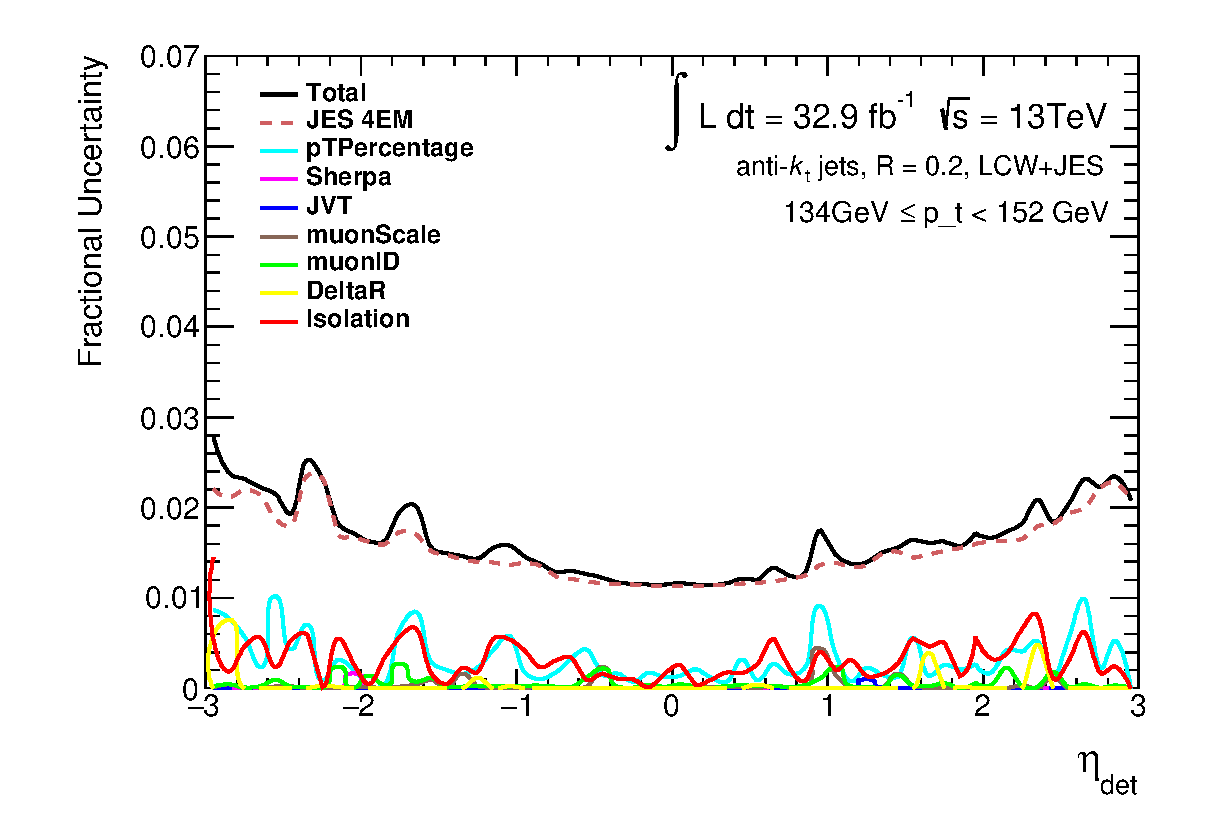
\includegraphics[width=\textwidth]{images/SumIn2_pT_10_2LC_wContributions.eps}
        \caption{$R=$0.2 ; 134GeV$<p^{Rscan}_t<$152GeV}
        %\label{fig:Th26lc}
    \end{subfigure}
    \vfill
    \begin{subfigure}[b]{0.495\textwidth}
        \centering
        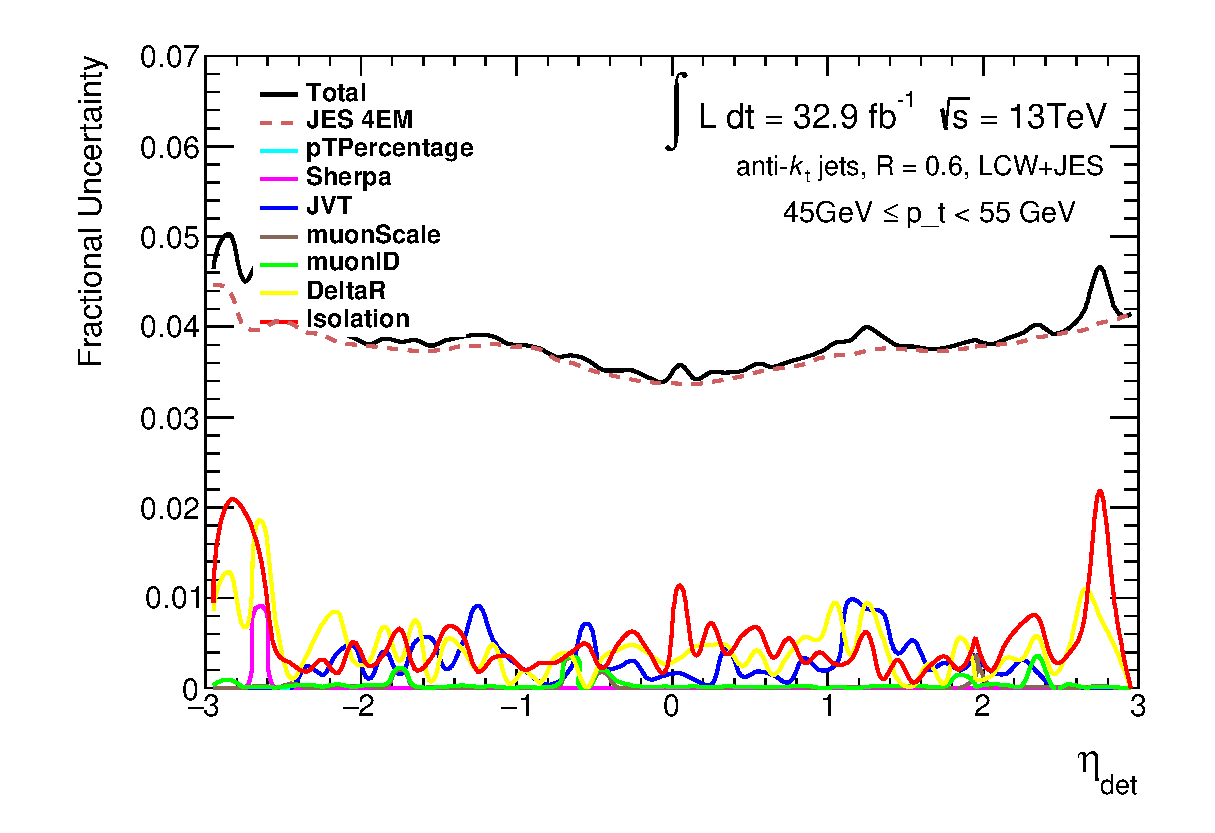
\includegraphics[width=\textwidth]{images/SumIn2_pT_4_6LC_wContributions.eps}
        \caption{$R=$0.6 ; 45GeV$<p_t^{Rscan}<$55GeV}
        %\label{fig:fitFeo}
    \end{subfigure}
    \hfill
    \begin{subfigure}[b]{0.495\textwidth}
        \centering
        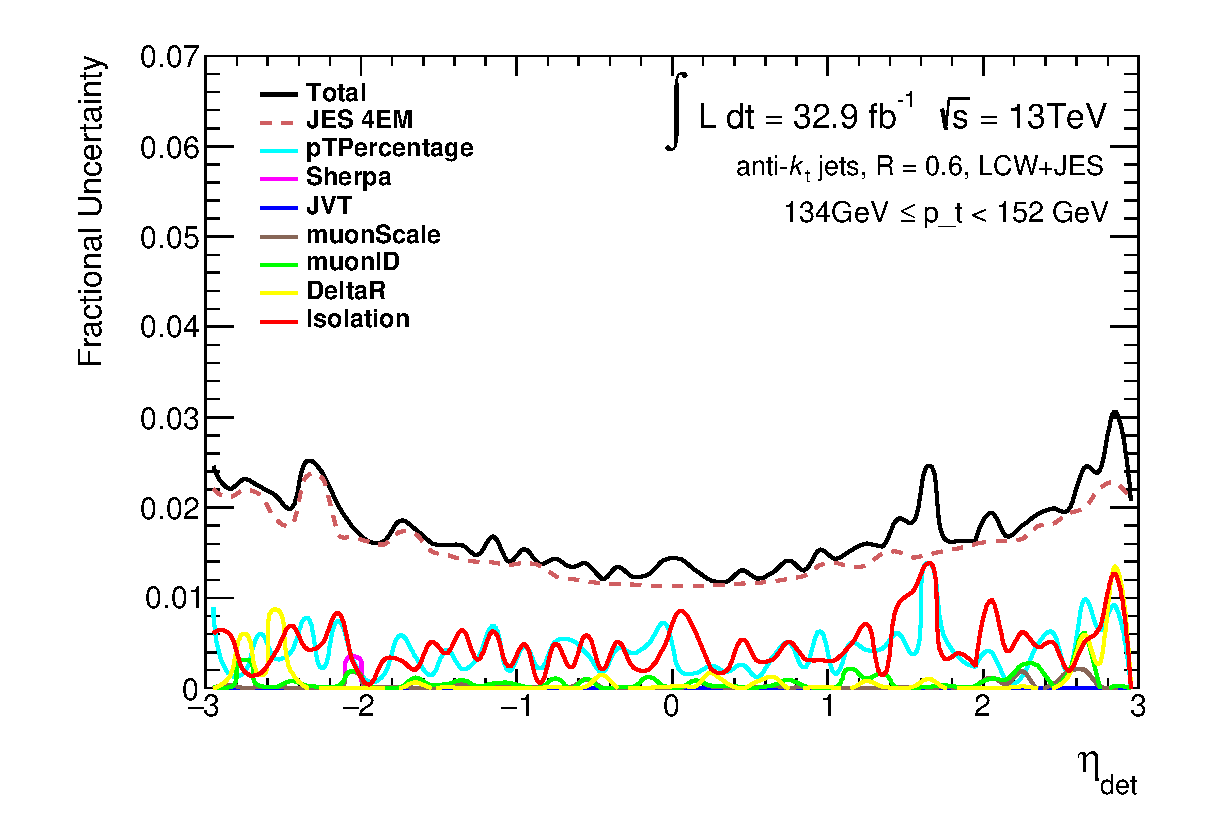
\includegraphics[width=\textwidth]{images/SumIn2_pT_10_6LC_wContributions.eps}
        \caption{$R=$0.6 ; 134GeV$<p^{Rscan}_t<$152GeV}
        %\label{fig:Th26lc}
    \end{subfigure}
    \caption{ Incerteza sistemática relativa total (en negro), y sus contribuciones, en función de $\eta_{det}$ en el bin de 45GeV$<p_t^{Rscan}<$55GeV a la derecha, y 134GeV$<p^{Rscan}_t<$152GeV a la izquierda. Las figuras superiores corresponden a la coelcción de Rscan Jets con $R=$0.2 y las inferiores a 0.6.} 
    \label{fig:UnvsEta}
\end{figure}

En la figura \ref{fig:UnvsEta} se observa la incerteza sistemática (relativa) total (en negro), en función $\eta_{det}$, y las contribuciones de cada parámetro estudiado a la misma, para dos bines de $p_t$ y para ambas colecciones de Rscan Jets. Nuevamente, se hace evidente en estas figuras que la contribución más significativa es la incerteza de las JES. Las incertezas correspondientes a las demás contribuciones muestran una gran variabilidad en la dirección de $\eta$. Dejando de lado esas fluctuaciones del orden del 1$\%$, se observa que la dependencia con $\eta$ de la incerteza total se hereda directamente de la contribución de la JES; y la misma es poco dependiente, manteniéndose del orden de alrededor del 4$\%$ a bajo momento, y más dependiente a alto momento, de casi un 3$\%$ en los bines de $\eta$ extremos y disminuyendo hasta el 1$\%$ hacia los bines centrales.\\


Finalmente, se presentan las calibraciones R-scan obtenidas en este trabajo para dos bines de $\eta$ en la figura \ref{fig:FinalCalibration}. Junto al factor de corrección se muestra la incerteza estadística y la incerteza total en función de $p_t^{Rscan}$.



\begin{figure}[ht]
    \centering
    \begin{subfigure}[b]{0.495\textwidth}
        \centering
        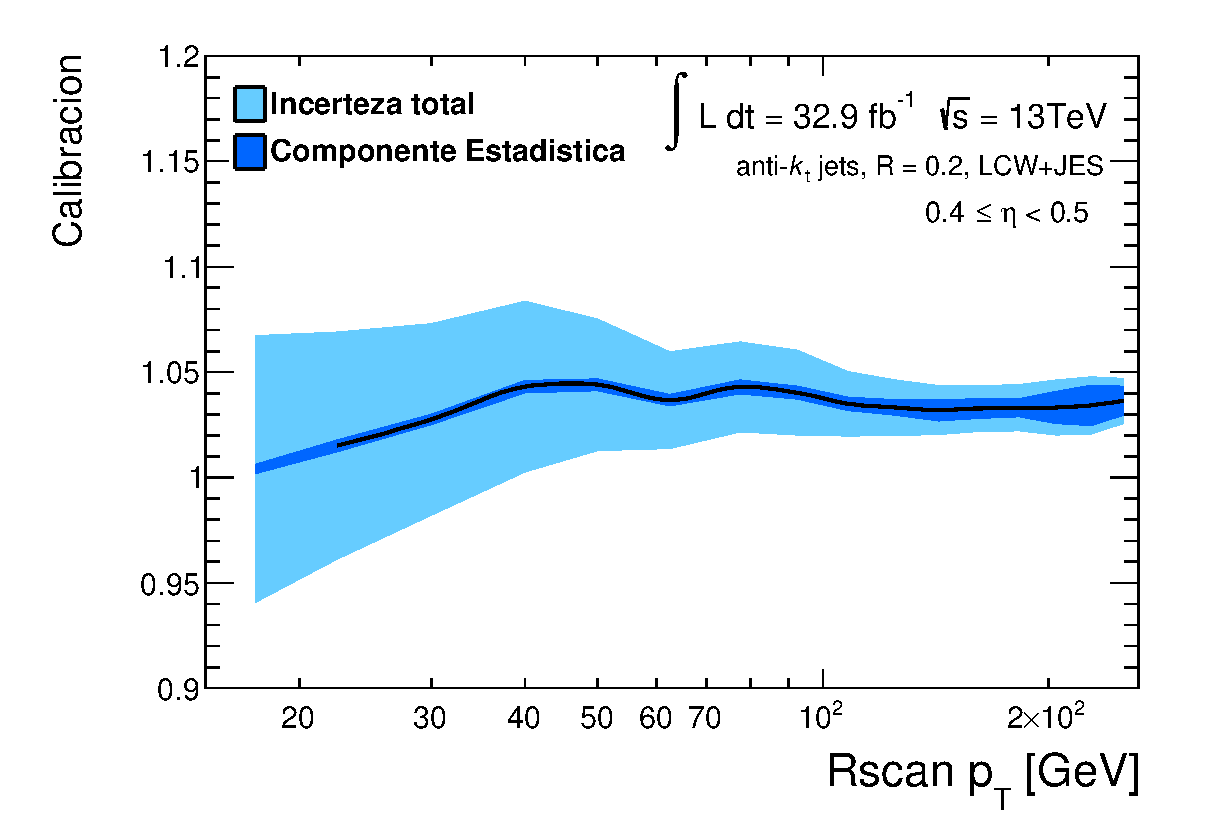
\includegraphics[width=\textwidth]{images/Final2LC/Calibration_Eta_49.eps}
        \caption{$R=$0.2 ; 0.4$<\eta^{Rscan}_{det}<$0.5}
        %\label{fig:data2lc49}
    \end{subfigure}
    \hfill
    \begin{subfigure}[b]{0.495\textwidth}
        \centering
        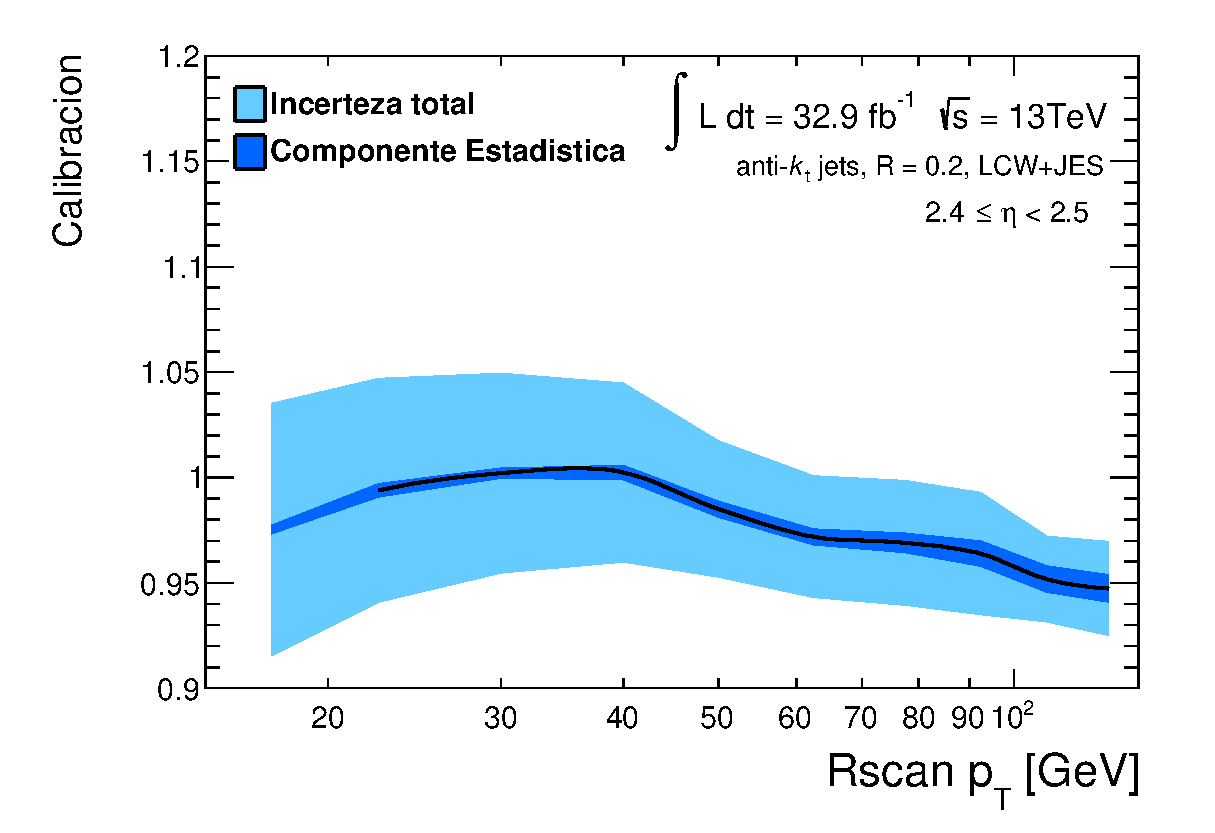
\includegraphics[width=\textwidth]{images/Final2LC/Calibration_Eta_69.eps}
        \caption{$R=$0.2 ; 2.4$<\eta^{Rscan}_{det}<$2.5}
        %\label{fig:Th26lc}
    \end{subfigure}
    \vfill
    \begin{subfigure}[b]{0.495\textwidth}
        \centering
        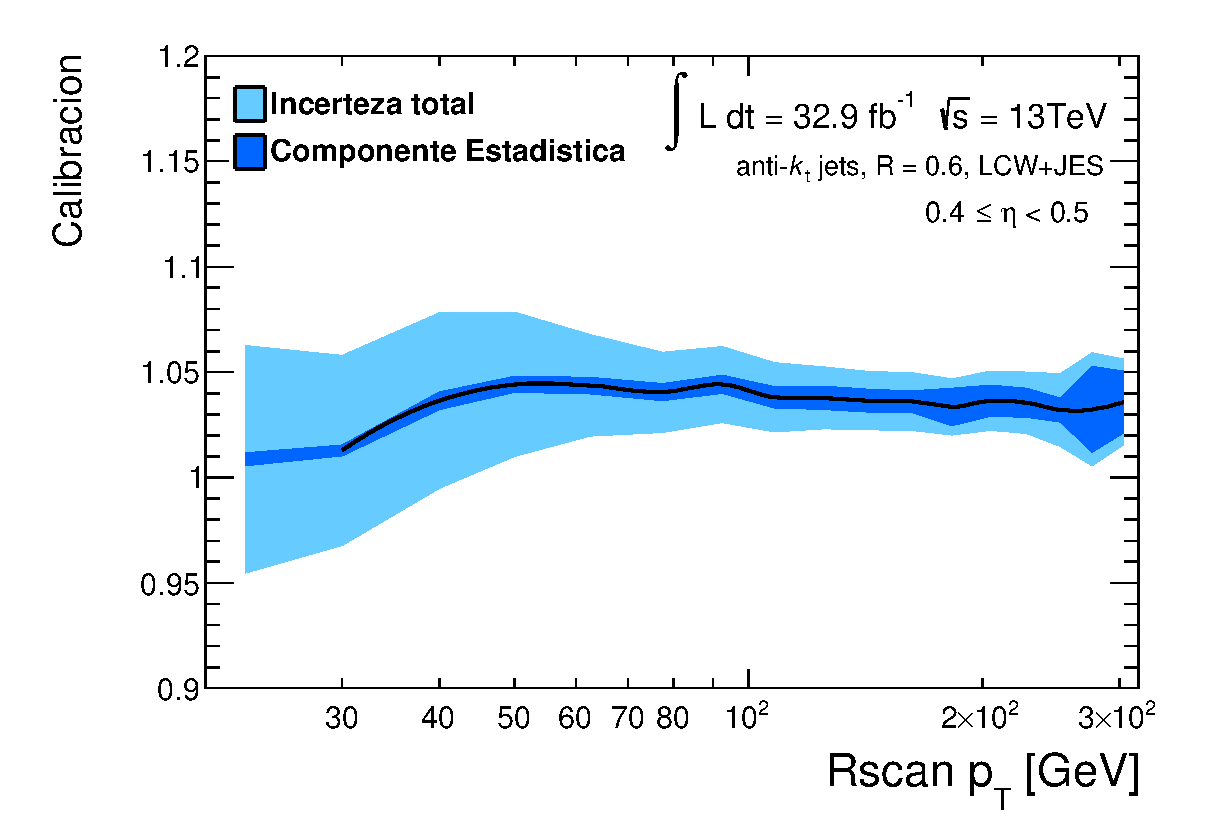
\includegraphics[width=\textwidth]{images/Final6LC/Calibration_Eta_49.eps}
        \caption{$R=$0.6 ; 0.4$<\eta^{Rscan}_{det}<$0.5}
        %\label{fig:fitFeo}
    \end{subfigure}
    \hfill
    \begin{subfigure}[b]{0.495\textwidth}
        \centering
        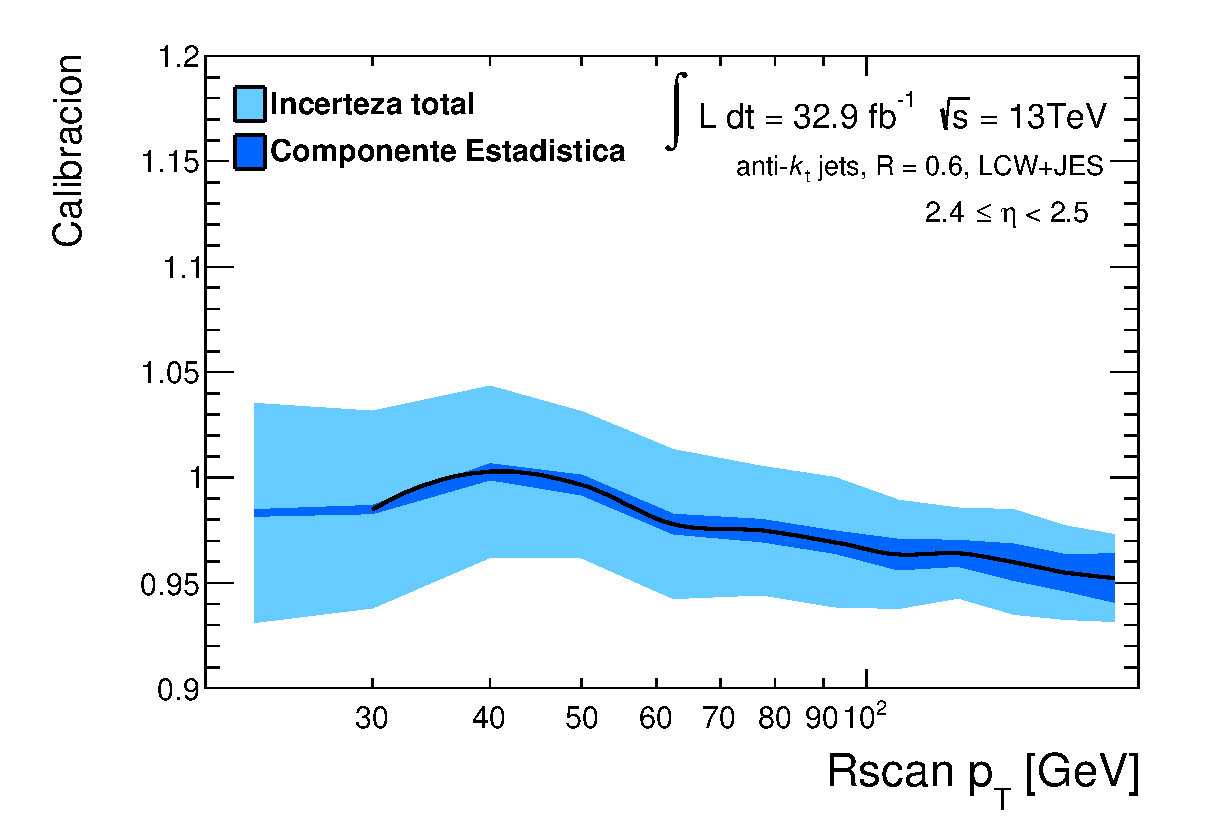
\includegraphics[width=\textwidth]{images/Final6LC/Calibration_Eta_69.eps}
        \caption{$R=$0.6 ; 2.4$<\eta^{Rscan}_{det}<$2.5}
        %\label{fig:Th26lc}
    \end{subfigure}
    \caption{ Calibración R-scan obtenida para Rscan Jets con $R=$ 0.2, (a) y (b) y 0.6 (c) y (d), en función de $p_t^{Rscan}$. Las figuras de la derecha corresponden al bin 2.4$<\eta^{Rscan}_{det}<$2.5 y las de la izquierda al bin 0.4$<\eta^{Rscan}_{det}<$0.5. En negro se muestra el calibración (suavizada); en celeste se muestra la incerteza total (suma en cuadratura de la componente estadística y la incerteza sistemática); y en azul más oscuro, la componente estadística de la incerteza.} 
    \label{fig:FinalCalibration}
\end{figure}



\afterpage{\null\newpage}